\documentclass[11pt,twoside,a4paper]{article}

\usepackage{hyperref}
\usepackage{graphicx}

\begin{document}
\title{AIML Homework 1}
\author{Matteo Borghesi}
\maketitle

\section{Dataset presentation}
In this report we are going to perform a shallow learning analysis on the wine dataset . 
%&\footnote{\url{https://scikit-learn.org/stable/modules/generated/sklearn.datasets.load_wine.html#examples-using-sklearn-datasets-load-wine}}
This dataset contains results of a chemical analysis of wines grown in the same region in Italy by three different cultivators. Although it features thirteen different measurements regarding different constituents, we will consider only two of them, which are the Alcohol and the Malic Acid. Our goal is to be able to predict which cultivator produced a certain wine just by looking at these two attributes.

In order to do that, we will randomly split the data in a training set, a validation set and a test set, with proportion 5:2:3. Since the dataset contains 178 samples overall, there will be 89 samples in the training set, 35 in the validation and 54 in the test set.
In section~\ref{CV} we will then merge the training and the validation set and proceed with cross validation on the resulting set.

In order to prevent one attribute from overpowering the other one in the analysis, the samples are normalized according to the mean and the variance computed on the training set only.

\section{K-nearest Neighbors}
As a first step, we apply the K-nearest Neighbors (a.k.a. KNN) algorithm to the Wine dataset. The idea behind said algorithm is to assign the class labels to the test items basing on their 'proximity' to the training samples. In particular, the label that occurs most often in the \emph{k} 'nearest' samples is chosen as prediction. The proximity between two samples can be measured according to different metrics: in our analysis - as it is mostly the case - we use the Euclidean distance, i.e. the norm of the difference between the two sample vectors.

We apply our analysis four times for different values of the parameter \emph{k} (respectively 1, 3, 5 and 7). The result of the training phase is shown in fig.~\ref{fig:knnPred}, with the dots representing the training items. The background colors on the other hand signal which class is assigned to test samples whose attributes fall within that area. As it can be seen on the plots, as \emph{k} increases the boundary lines become more uniform, since they depend less on single or few samples lying in a area where the majority of the items belong to a different class. Although this reduces the risk of overfitting the data provided, it may also reduce the model's capability of recognizing particular structures in the data.
Indeed, if we measure the accuracy of the model to varying of \emph{k} we notice that it's not necessarily the highest \emph{k} that makes the best prediction (see fig.~\ref{fig:knnScore}). This balance between overfitting and underfitting the data, known as bias-variance tradeoff, is inherent to most statistical learning methods.\newline
As intuition suggests, we choose as optimal the value of \emph{k} that maximizes the accuracy of the model on the validation test. Once we have done that, we can estimate the reliability of the model by measuring its accuracy on the test set, whose data have been kept out during all through the process of model selection. Clearly, the accuracy measured both on the validation and on the test set depends on the split performed during the first stage, which we said to be random: the smaller are the sets, the higher is the variance of these measures. With the split made in the beginning, test accuracy turns out to be XXX.

\begin{figure}[]
  \begin{center}
  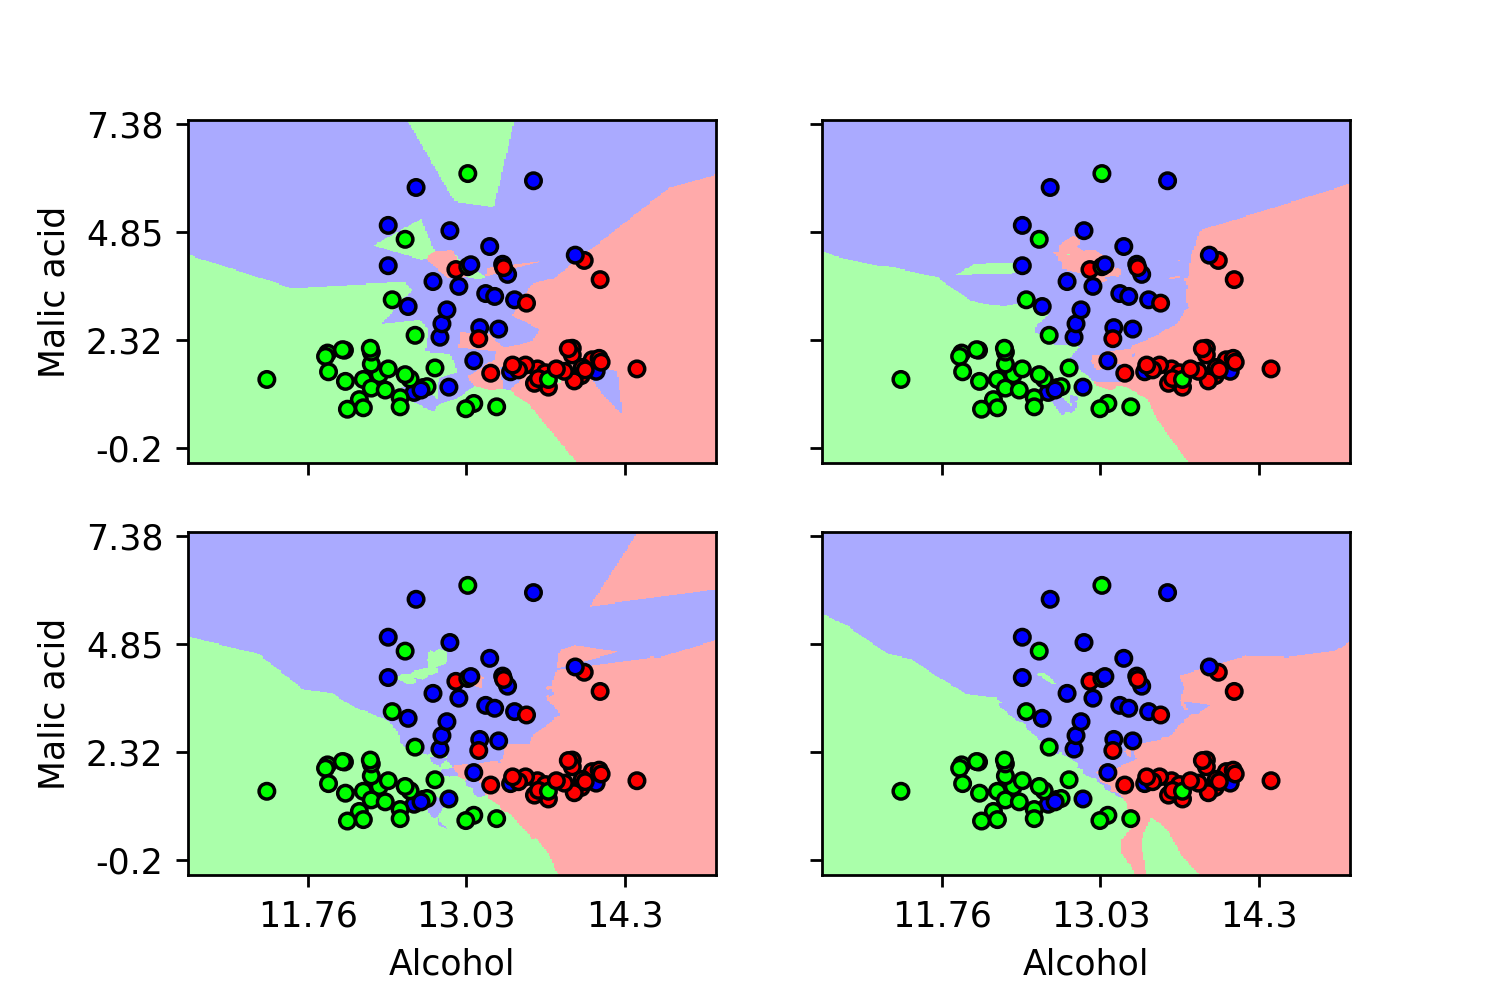
\includegraphics[]{knnPredPlot.png}
  \caption{Knn analysis}
  \label{fig:knnPred}
  \end{center}
\end{figure}

\begin{figure}[]
  \begin{center}
  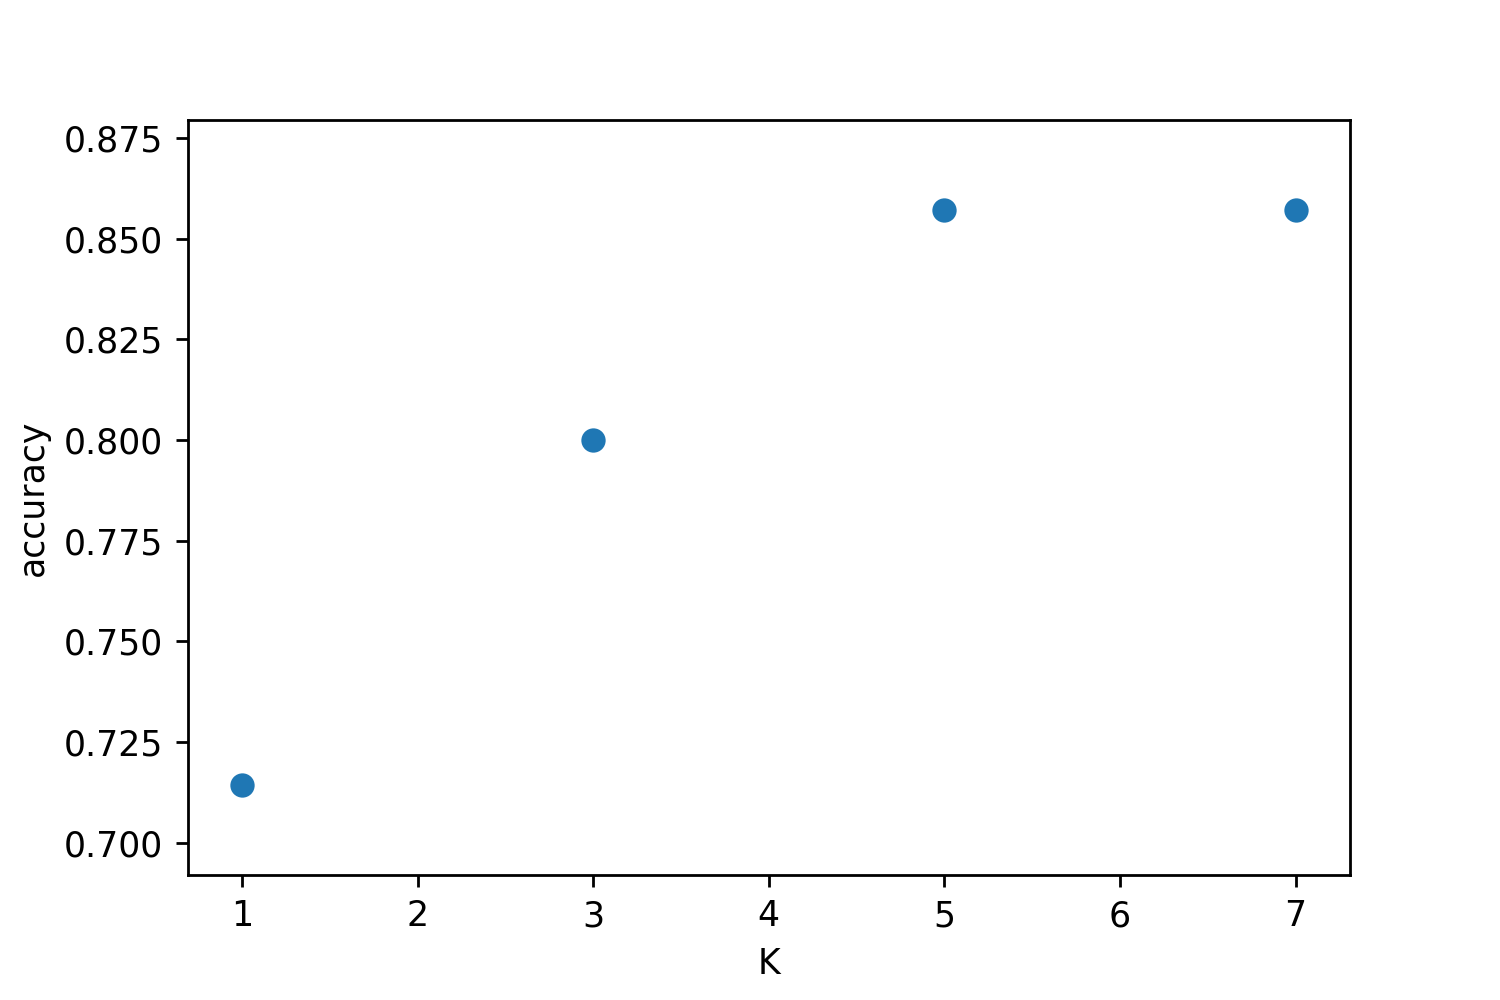
\includegraphics[]{knnScorePlot.png}
  \caption{Knn accuracy}
  \label{fig:knnScore}
  \end{center}
\end{figure}

\section{Linear Support Vector Machines}
In the second stage of our classification analysis, we use a method called Support Vector Machines (SVM), which aims to find linear decision boundaries in the plane of the feature vectors, so that all points belonging to the same class lie on the same side of the boundary. Furthermore, SVM is designed to maximize the minimum distance between the linear separator and the points of all classes.\newline
If the problem is not linearly separable, it is possible to introduce a parameter \emph{C} in the model, called 'slack variable', which tells how far beyond the decision boundary the points are allowed to be in case they fall into the area of another class.

As we already did for KNN, we build classifiers for multiple values of \emph{C} (here 0.001, 0.01, 0.1, 1, 10, 100, 1000) basing on the training set and evaluate them on the validation set, then we choose the one with the best score and assess its reliability by means of the test set.

\section{CV}
\label{CV}
lorem ipsum


\end{document}

